\documentclass[paper=a4, fontsize=11pt]{scrartcl} % A4 paper and 11pt font size
\usepackage[utf8]{inputenc}

\usepackage[T1]{fontenc} % Use 8-bit encoding that has 256 glyphs
\usepackage{fourier} % Use the Adobe Utopia font for the document - comment this line to return to the LaTeX default
\usepackage[english]{babel} % English language/hyphenation
\usepackage{amsmath,amsfonts,amsthm} % Math packages
\usepackage{mathtools}

\usepackage{lipsum} % Used for inserting dummy 'Lorem ipsum' text into the template

\usepackage{sectsty} % Allows customizing section commands
\allsectionsfont{\centering \normalfont\scshape} % Make all sections centered, the default font and small caps
\usepackage{graphicx}
\usepackage{breqn}

\usepackage{fancyhdr} % Custom headers and footers
\pagestyle{fancyplain} % Makes all pages in the document conform to the custom headers and footers
\fancyhead{} % No page header - if you want one, create it in the same way as the footers below
\fancyfoot[L]{} % Empty left footer
\fancyfoot[C]{} % Empty center footer
\fancyfoot[R]{\thepage} % Page numbering for right footer
\renewcommand{\headrulewidth}{0pt} % Remove header underlines
\renewcommand{\footrulewidth}{0pt} % Remove footer underlines
\setlength{\headheight}{13.6pt} % Customize the height of the header


\setlength\parindent{0pt} % Removes all indentation from paragraphs - comment this line for an assignment with lots of text

%----------------------------------------------------------------------------------------
%	TITLE SECTION
%----------------------------------------------------------------------------------------

\newcommand{\horrule}[1]{\rule{\linewidth}{#1}} % Create horizontal rule command with 1 argument of height

\title{	
	\normalfont \normalsize 
	\textsc{Aarhus Universitet, Science, datalogi} \\ [25pt] % Your university, school and/or department name(s)
	\horrule{0.5pt} \\[0.4cm] % Thin top horizontal rule
	\huge Assignment Title \\ % The assignment title
	\horrule{2pt} \\[0.5cm] % Thick bottom horizontal rule
}

\author{Peter Burgaard - 201209175} % Your name

\date{\normalsize\today} % Today's date or a custom date

\begin{document}
	
	\maketitle % Print the title
	
	Vi har følgende variabler og konstanter:
	\begin{align*}
	x_i &= \text{vægt for produkt i, og den eneste variable} \\
	p_i &= \text{pris for produkt i} \\
	a_{Pi} &= \text{proteindhold i produkt i} \\
	a_{Fi} &= \text{fedtindhold i produkt i} \\
	a_{Ki} &= \text{kulhydratindt i produkt i} \\
	a_{Ei} &= \text{samlede energi i KJ for produkt i} 
	\end{align*}
	
	vi har udarbejdet ud fra følgende varer:
	\begin{figure}
		\centering
		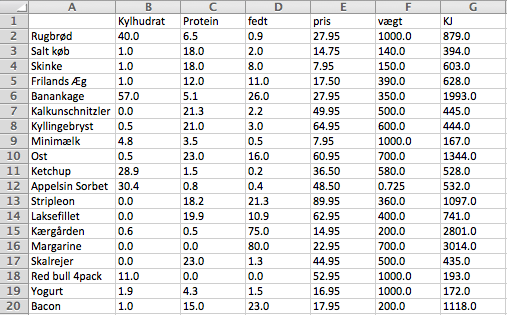
\includegraphics[width=9cm]{tabel.png}
	\end{figure}
	
	med følgende objective function og constraints:
	\begin{align*}
	& \text{Max } &&\zeta = \sum_{i=1}^{n} x_i*p_i \\
	&\text{Engergi} \hspace{3cm} \text{s.t.} &&10000 \leq \sum_{i=1}^{n}x_i*a_{Ei}   \\
	&\text{Protein} \hspace{3cm} && \sum_{i=1}^{n}x_i*a_{Pi}*17 \leq 0.25*\sum_{i=1}^{n}x_i*a_{Ei} \\
	& && 0.10*\sum_{i=1}^{n}x_i*a_{Ei} \leq \sum_{i=1}^{n}x_i*a_{Pi}*17 \\
	& \text{Kulhydrater} &&  \sum_{i=1}^{n}x_i*a_{Ki}*17 \leq 0.60*\sum_{i=1}^{n}x_i*a_{Ei}\\
	& && 0.55*\sum_{i=1}^{n}x_i*a_{Ei} \leq \sum_{i=1}^{n}x_i*a_{Ki}*17 \\
	& \text{Fedt} &&  \sum_{i=1}^{n}x_i*a_{Ki}*38 \leq 0.30*\sum_{i=1}^{n}x_i*a_{Ei}\\
	& && 0.2*\sum_{i=1}^{n}x_i*a_{Ei} \leq \sum_{i=1}^{n}x_i*a_{Fi}*38 \\
	\end{align*}
	
	Nogle af disse constraints er vendt rundt når de indsættes i programmet.
	Hvilket giver følgende input, results i terminalen, og resultat ift fødevare

	\begin{figure}
		\centering
		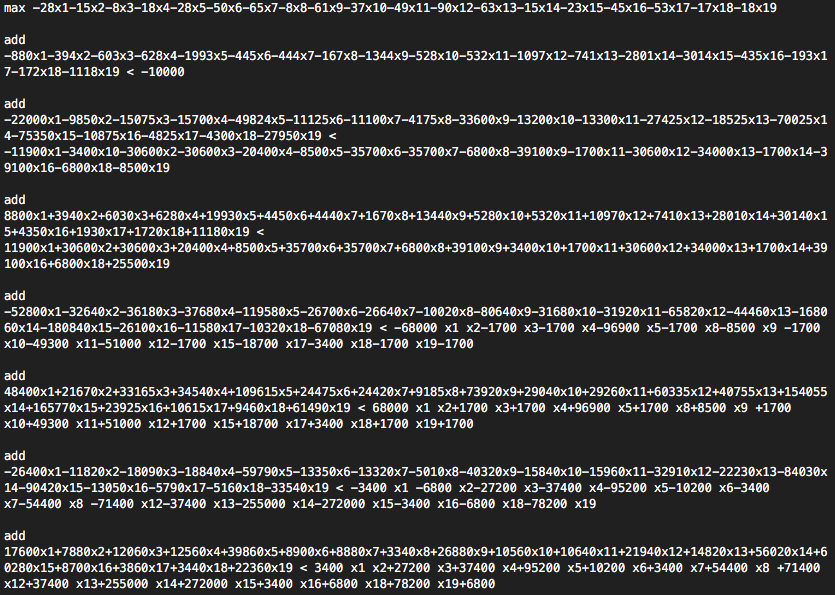
\includegraphics[width=\textwidth]{table.png}
	\end{figure}

	
	\begin{figure}
		\centering
		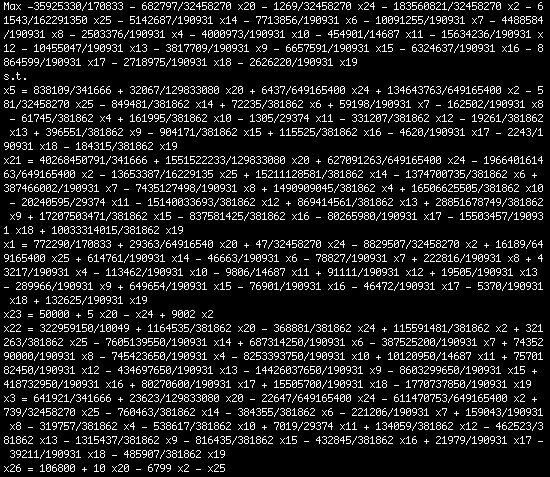
\includegraphics[width=10cm]{result.png}
	\end{figure}
	
	\begin{figure}
		\centering
		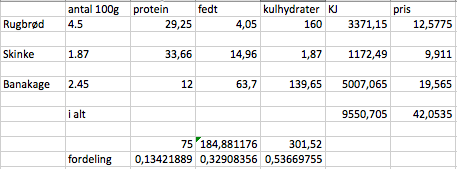
\includegraphics[width=10cm]{solution.png}
	\end{figure}

\end{document}
